\documentclass[11pt,a4paper]{article}
\usepackage[utf8]{inputenc}
\usepackage[margin=2.2cm]{geometry}
\usepackage{graphicx,booktabs,amsmath,amssymb,hyperref,xcolor,listings,float,enumitem,caption,multirow}
\usepackage{tikz}
\usetikzlibrary{shapes.geometric,arrows.meta,positioning,calc,fit,backgrounds}

\hypersetup{colorlinks=true,linkcolor=blue,urlcolor=blue}
\lstset{language=C,basicstyle=\ttfamily\small,keywordstyle=\color{blue}\bfseries,
  commentstyle=\color{gray},numbers=left,numberstyle=\tiny\color{gray},
  breaklines=true,frame=single,tabsize=4,captionpos=b}

\title{\textbf{Project 3: High-Performance Matrix Multiplication in C}\\[0.4em]
\large From 0.69 to 385 GFLOPS on Apple M5 --- A 558$\times$ Speedup}
\author{Name: Lunhan Yan \quad Student ID: 12412823}
\date{May 2026}

\begin{document}
\maketitle

\section{Introduction}

Matrix multiplication $C=A\times B$ is the computational core of deep learning.
This project implements single-precision (\texttt{float}) matrix multiplication in C
and optimizes it through six phases, achieving \textbf{385 GFLOPS} at $8192^2$
(75\% of OpenBLAS) with a \textbf{558$\times$} speedup over the na\"ive baseline.

\textbf{Platforms:}
\begin{itemize}[nosep]
  \item \textbf{Local:} Apple M5 MacBook Air --- 4P+6E cores, 16\,GB RAM
  \item \textbf{Cloud:} Alibaba Cloud \texttt{g8y.8xlarge} --- 32-core ARM (Yitian 710), 122\,GB (for 64K)
\end{itemize}

\subsection*{Code Structure}

The project is organized into three source files:

\begin{table}[H]\centering
\begin{tabular}{l|l}
\toprule
\textbf{File} & \textbf{Role} \\
\midrule
\texttt{matrix.h} & Single-header library: \texttt{Matrix} struct and utility functions \\
                   & (\texttt{matrix\_create}, \texttt{matrix\_free}, \texttt{matrix\_random}, \texttt{matrix\_zero}, etc.) \\
\texttt{matmul\_plain.c} & Baseline $i$-$j$-$k$ implementation + benchmark driver (\texttt{main}) \\
\texttt{matmul\_improved.c} & Optimized BLIS-style implementation (NEON SIMD + OpenMP) \\
\bottomrule
\end{tabular}
\end{table}

\noindent\textbf{Compilation (macOS):}
\begin{lstlisting}[language=bash,numbers=none,basicstyle=\ttfamily\scriptsize]
gcc -O3 -Xpreprocessor -fopenmp -I$(brew --prefix libomp)/include \
    -L$(brew --prefix libomp)/lib -lomp -I$(brew --prefix openblas)/include \
    -L$(brew --prefix openblas)/lib -lopenblas \
    -o benchmark matmul_plain.c matmul_improved.c -lm
\end{lstlisting}

\section{Implementation}

\subsection{Baseline: \texttt{matmul\_plain}}

Standard $i$-$j$-$k$ loops. Inner loop accesses \texttt{B[k][j]} with stride $n$,
causing heavy cache misses. Achieves \textbf{2.0 GFLOPS} at $1024^2$
and only \textbf{0.69 GFLOPS} at $8192^2$.

\subsection{Optimized: \texttt{matmul\_improved} --- Six Phases}

% ── Roadmap Flowchart ──
\begin{figure}[H]
\centering
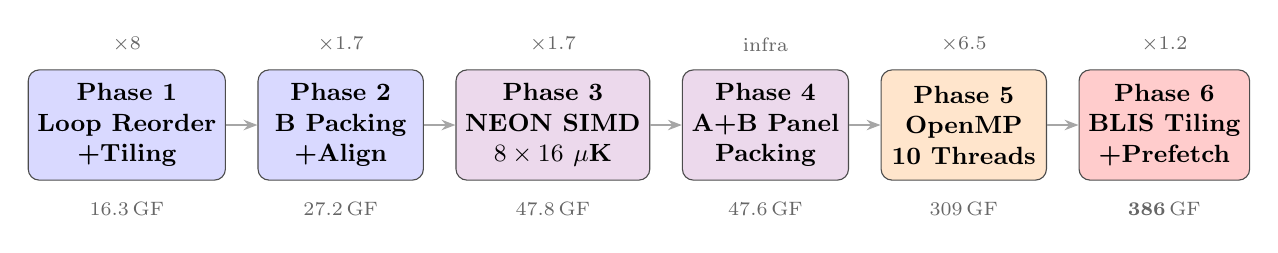
\begin{tikzpicture}[
  phase/.style={rectangle, rounded corners=4pt, draw=black!70, fill=#1,
    minimum width=2.1cm, minimum height=1.4cm, align=center, font=\small\bfseries},
  arr/.style={-{Stealth[length=5pt]}, thick, gray!70},
  res/.style={font=\scriptsize\color{black!60}, align=center}
]
\node[phase=blue!15]   (p1) {Phase 1\\Loop Reorder\\+Tiling};
\node[phase=blue!15,   right=0.4cm of p1] (p2) {Phase 2\\B Packing\\+Align};
\node[phase=violet!15, right=0.4cm of p2] (p3) {Phase 3\\NEON SIMD\\$8\times16$ $\mu$K};
\node[phase=violet!15, right=0.4cm of p3] (p4) {Phase 4\\A+B Panel\\Packing};
\node[phase=orange!20, right=0.4cm of p4] (p5) {Phase 5\\OpenMP\\10 Threads};
\node[phase=red!20,    right=0.4cm of p5] (p6) {Phase 6\\BLIS Tiling\\+Prefetch};

\foreach \n/\v in {p1/16.3,p2/27.2,p3/47.8,p4/47.6,p5/309,p6/\textbf{386}} {
  \node[res, below=0.15cm of \n] {\v\,GF};
}
\draw[arr] (p1)--(p2); \draw[arr] (p2)--(p3); \draw[arr] (p3)--(p4);
\draw[arr] (p4)--(p5); \draw[arr] (p5)--(p6);

\node[res, above=0.1cm of p1] {$\times8$};
\node[res, above=0.1cm of p2] {$\times1.7$};
\node[res, above=0.1cm of p3] {$\times1.7$};
\node[res, above=0.1cm of p4] {infra};
\node[res, above=0.1cm of p5] {$\times6.5$};
\node[res, above=0.1cm of p6] {$\times1.2$};
\end{tikzpicture}
\caption{Optimization roadmap (GFLOPS at $8192^2$, speedup relative to previous phase).}
\end{figure}

\subsubsection{Phase 1: Loop Reordering + Cache Tiling}

\textbf{Problem:} $i$-$j$-$k$ order $\Rightarrow$ stride-$n$ access on B $\Rightarrow$ cache miss $>50\%$.

\textbf{Solution:} Reorder to $i$-$k$-$j$ (stride-1 on both B and C) + $64\times64$ tiling.

The outer loop nest partitions the matrix into tiles:
\begin{lstlisting}[language={},basicstyle=\ttfamily\scriptsize,frame=single,numbers=none]
for ii = 0..m step 64          // tile rows of A and C
  for kk = 0..k step 64        // tile the shared dimension
    for jj = 0..n step 64      // tile columns of B and C
      i-k-j loop on the 64x64 sub-blocks
\end{lstlisting}

\textbf{Cache addressing (M5 L1):}
128\,KB, 8-way, line $L{=}128$\,B, sets $S{=}128$.
A byte at address $a$ maps to set $\lfloor a/L \rfloor \bmod S$;
each set holds at most 8 lines (ways).

\textbf{Explanation:}
Without tiling, the inner $j$-loop sweeps an entire row of B and C ($N$ elements = $N/32$ cache lines each).
These lines occupy $N/32 \bmod S$ sets; at $N{=}8192$ that is 256 lines spread over 128 sets, so B and C together load $\sim$4 lines per set---manageable in isolation, but the \emph{full matrix B} ($N^2$ elements, 256\,MB) must be re-streamed from DRAM for every row $i$.
Tiling with $T{=}64$ confines each tile to $T/32{=}2$ lines per set and---critically---lets each $T{\times}T$ B-tile (16\,KB) be reused across $T$ rows of $i$ while staying in L1, cutting total DRAM traffic by $\sim T{\times}$.

% ── Tiling diagram ──
\begin{figure}[H]
\centering
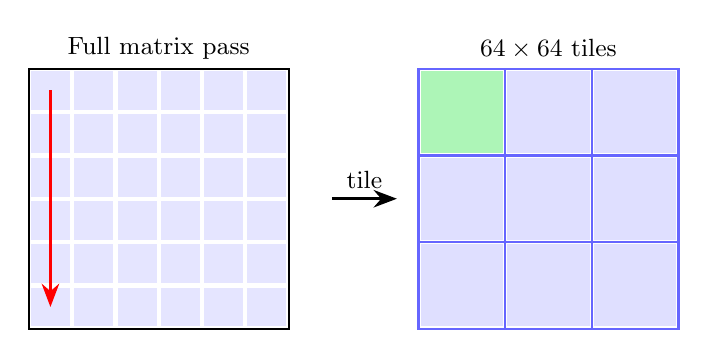
\begin{tikzpicture}[scale=0.55]
  % Left: no tiling
  \draw[thick] (0,0) rectangle (6,6);
  \foreach \i in {0,...,5} \foreach \j in {0,...,5}
    \fill[blue!10] (\j+0.05,\i+0.05) rectangle (\j+0.95,\i+0.95);
  \draw[-{Stealth},red,very thick] (0.5,5.5)--(0.5,0.5);
  \node[above] at (3,6) {\small Full matrix pass};

  % Arrow
  \draw[-{Stealth},very thick] (7,3)--(8.5,3);
  \node[above] at (7.75,3) {\small tile};

  % Right: tiled
  \draw[thick] (9,0) rectangle (15,6);
  \foreach \i in {0,2,4} \foreach \j in {0,2,4} {
    \draw[blue!60,thick] (9+\j,\i) rectangle (9+\j+2,\i+2);
    \fill[blue!25,opacity=0.5] (9+\j+0.05,\i+0.05) rectangle (9+\j+1.95,\i+1.95);
  }
  \fill[green!40,opacity=0.7] (9.05,4.05) rectangle (10.95,5.95);
  \node[above] at (12,6) {\small $64\times64$ tiles};
\end{tikzpicture}
\caption{Cache tiling: partition into L1-sized blocks.}
\end{figure}

\textbf{Result:} 16.3 GFLOPS at $8192^2$ ($\times$8.2 vs baseline).

\subsubsection{Phase 2: B-Matrix Packing + Alignment}

\textbf{Problem:} B columns map to same cache sets $\Rightarrow$ conflict misses.

\textbf{Solution:} Copy B sub-block into a contiguous, 128-byte-aligned buffer before computation.
\textbf{Explanation:}
The L1 set index is $\lfloor\text{addr}/L\rfloor \bmod S$. In row-major B, adjacent rows at the same column differ by stride $N{\times}4$\,B, giving a set step of $(N/32)\bmod 128$. When $N$ is a multiple of 4096 this equals 0---all rows hit the \emph{same} set and thrash the 8 ways.
Packing copies the tile into contiguous memory with stride $T{\times}4$; at $T{=}64$ the set step becomes 2, spreading rows across 64 distinct sets and eliminating conflicts.

\begin{lstlisting}[caption={B packing}]
float packed_B[TILE*TILE] __attribute__((aligned(128)));
for (k = 0; k < tile_k; k++)
    for (j = 0; j < tile_n; j++)
        packed_B[k*tile_n + j] = B[(kk+k)*n + jj+j];
\end{lstlisting}

\textbf{Result:} 27.2 GFLOPS at $8192^2$ ($\times$1.7).

\subsubsection{Phase 3: NEON SIMD + $8\times16$ Micro-Kernel}

\textbf{Problem:} Scalar FMA = 1 FLOP/instr. NEON can do 4.

\textbf{Solution:} $8\times16$ micro-kernel using all 32 AArch64 NEON registers.
Within each $64{\times}64$ tile, we further partition into $8{\times}16$ sub-blocks
for register-level blocking:
\begin{lstlisting}[language={},basicstyle=\ttfamily\scriptsize,frame=single,numbers=none]
for ii, kk, jj (step 64)       // same outer tiling as before
  for ir = 0..64 step MR=8     // sub-tile rows (8 rows per micro-kernel)
    for jr = 0..64 step NR=16  // sub-tile cols (16 cols per micro-kernel)
      micro_kernel_8x16(A[ii+ir..], B[kk..][jj+jr..], C[ii+ir..][jj+jr..])
\end{lstlisting}

% ── Outer-product (rank-1 update) diagram ──
\begin{figure}[H]
\centering
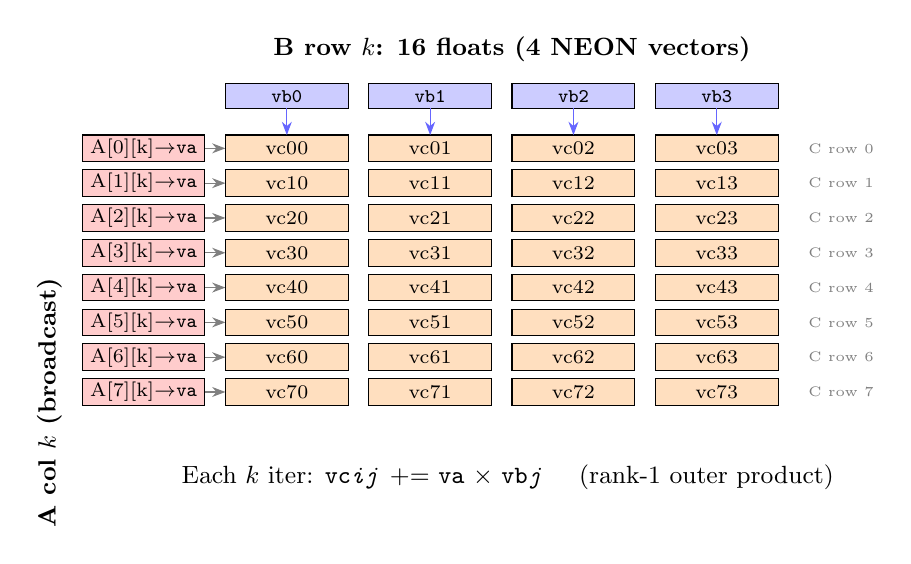
\begin{tikzpicture}[scale=0.52, every node/.style={font=\scriptsize}]
  % B row (top) — 4 vectors
  \foreach \j/\lbl in {0/vb0,1/vb1,2/vb2,3/vb3} {
    \fill[blue!20] (\j*3.5+2, 1.2) rectangle (\j*3.5+5, 1.8);
    \draw (\j*3.5+2, 1.2) rectangle (\j*3.5+5, 1.8);
    \node at (\j*3.5+3.5, 1.5) {\texttt{\lbl}};
  }
  \node[above,font=\small\bfseries] at (9, 2.1) {B row $k$: 16 floats (4 NEON vectors)};

  % A column (left) — 8 scalars
  \foreach \i in {0,...,7} {
    \fill[red!20] (-1.5, -\i*0.85+0.55) rectangle (1.5, -\i*0.85-0.1);
    \draw (-1.5, -\i*0.85+0.55) rectangle (1.5, -\i*0.85-0.1);
    \node at (0, -\i*0.85+0.225) {A[\i][k]$\to$\texttt{va}};
    % Arrow from A to C row
    \draw[-{Stealth},gray,thin] (1.5, -\i*0.85+0.225) -- (2, -\i*0.85+0.225);
  }
  \node[left,font=\small\bfseries,align=center,rotate=90] at (-2.3, -2.7) {A col $k$ (broadcast)};

  % C block — 8 rows × 4 columns of accumulators
  \foreach \i in {0,...,7} {
    \foreach \j in {0,...,3} {
      \fill[orange!25] (\j*3.5+2, -\i*0.85+0.55) rectangle (\j*3.5+5, -\i*0.85-0.1);
      \draw (\j*3.5+2, -\i*0.85+0.55) rectangle (\j*3.5+5, -\i*0.85-0.1);
      \node at (\j*3.5+3.5, -\i*0.85+0.225) {vc\i\j};
    }
    % Row label
    \node[right,font=\tiny,gray] at (16, -\i*0.85+0.225) {C row \i};
  }

  % Vertical arrows from B to C columns
  \foreach \j in {0,...,3} {
    \draw[-{Stealth},blue!60,thin] (\j*3.5+3.5, 1.2) -- (\j*3.5+3.5, 0.55);
  }

  % Caption equation
  \node[font=\small,align=center] at (9, -7.8) {
    Each $k$ iter: \texttt{vc\textit{ij}} += \texttt{va} $\times$ \texttt{vb\textit{j}} \quad (rank-1 outer product)
  };
\end{tikzpicture}
\caption{One $k$ iteration: A's column is broadcast and multiplied with B's row, updating all 32 C accumulators.}
\end{figure}

\begin{lstlisting}[caption={Micro-kernel core (one $k$ iter, row 0)}]
float32x4_t vb0 = vld1q_f32(bp);       // B[k][j:j+3]
float32x4_t va  = vdupq_n_f32(ap[0]);  // broadcast A[0][k]
vc00 = vfmaq_f32(vc00, va, vb0);       // C[0][0:3] += A[0][k]*B[k][0:3]
\end{lstlisting}

\textbf{Explanation:}
Two orthogonal optimizations work together here.
\emph{NEON vectorization} widens each FMA from 1 to 4 floats per instruction, increasing compute throughput.
\emph{Register tiling} ($8{\times}16$ sub-blocks within the $64{\times}64$ cache tile) keeps the C sub-block pinned in registers across the entire $k$ loop, reducing C's load/store from once-per-$k$ to once-total.
Without register tiling, load/store ports become the bottleneck (FMA utilization ${\sim}50\%$); with it, the FMA units run at near-100\% utilization.

\textbf{Result:} 47.8 GFLOPS at $8192^2$ ($\times$1.7).



\subsubsection{Phase 4: A+B Panel Packing}

\textbf{Problem:} The micro-kernel reads A column-wise
(\texttt{A[0][k], A[1][k], \ldots, A[7][k]}), but A is row-major
with stride $lda$---8 values scattered across 8 rows, causing cache conflicts.

\textbf{Solution (A --- compact + transpose):}
After $ii$ and $kk$ are fixed, the entire $64{\times}64$ A tile is packed into
\texttt{packed\_A}: row-major (stride $lda$) $\to$ column-major strips (stride $MR{=}8$),
so each group of 8 floats from the same column becomes contiguous.
Packed \emph{once per $(ii, kk)$}, reused across all $jj$ (A does not depend on $j$).

\textbf{Solution (B --- slicing into strips):}
After $jj$ and $jr$ are fixed, the $kc{\times}16$ strip of B is copied into
\texttt{packed\_B} (stride $n \to$ stride $NR{=}16$).
The same strip is reused by all $ir$ iterations (B does not depend on $i$).

% ── Phase 4 computation diagram ──
\begin{figure}[H]
\centering
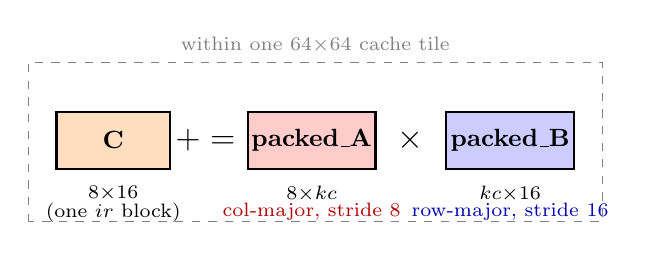
\begin{tikzpicture}[scale=0.45, every node/.style={font=\small}]
  % C sub-block 8×16
  \fill[orange!25] (0,0) rectangle (3.2,1.6);
  \draw[thick] (0,0) rectangle (3.2,1.6);
  \node at (1.6,0.8) {\textbf{C}};
  \node[below,font=\scriptsize] at (1.6,-0.2) {$8{\times}16$};
  \node[below,font=\scriptsize] at (1.6,-0.7) {(one $ir$ block)};
  % +=
  \node[font=\large\bfseries] at (4.2, 0.8) {$+=$};
  % packed_A panel
  \fill[red!20] (5.4,0) rectangle (9,1.6);
  \draw[thick] (5.4,0) rectangle (9,1.6);
  \node at (7.2,0.8) {\textbf{packed\_A}};
  \node[below,font=\scriptsize] at (7.2,-0.2) {$8{\times}kc$};
  \node[below,font=\scriptsize,red!70!black] at (7.2,-0.7) {col-major, stride 8};
  % ×
  \node[font=\large\bfseries] at (10, 0.8) {$\times$};
  % packed_B strip
  \fill[blue!20] (11,0) rectangle (14.6,1.6);
  \draw[thick] (11,0) rectangle (14.6,1.6);
  \node at (12.8,0.8) {\textbf{packed\_B}};
  \node[below,font=\scriptsize] at (12.8,-0.2) {$kc{\times}16$};
  \node[below,font=\scriptsize,blue!70!black] at (12.8,-0.7) {row-major, stride 16};
  % Context
  \draw[dashed,gray] (-0.8,-1.5) rectangle (15.4,3);
  \node[above,font=\scriptsize,gray] at (7.3,3) {within one $64{\times}64$ cache tile};
\end{tikzpicture}
\caption{Micro-kernel view: C[8$\times$16] += packed\_A[8$\times$kc] $\times$ packed\_B[kc$\times$16].}
\end{figure}

Infrastructure for Phase~6. 
\textbf{Result:} 47.6 GFLOPS (holds steady---packing
overhead offsets conflict reduction at $64^2$; payoff comes with larger BLIS blocks).

\subsubsection{Phase 5: OpenMP Multi-Threading}

\textbf{Problem:} Single-core NEON peak $\approx$ 61 GFLOPS. M5 has 10 cores.

\textbf{Solution:} \texttt{\#pragma omp parallel for} on the outermost row loop.
Each thread owns distinct C rows + stack-allocated private packing buffers (zero locks).

\begin{table}[H]\centering
\begin{tabular}{l|rr|r}
\toprule Threads & @$1024^2$ & @$8192^2$ & Speedup (8K) \\
\midrule
1 (baseline)   & 58.9  & 47.6  & 1.0$\times$ \\
4 (P-cores)    & 191.4 & 176.3 & 3.7$\times$ \\
10 (all cores) & 267.8 & 309.0 & 6.5$\times$ \\
\bottomrule
\end{tabular}
\caption{Thread scaling. 4P-cores near-linear; 6 E-cores add $\sim$2.4$\times$ equivalent.}
\end{table}

\subsubsection{Phase 6: BLIS Multi-Level Tiling + Prefetch}

\textbf{Problem:} Fixed $64^2$ tiling doesn't match the 3-level cache hierarchy.

\textbf{Loop structure evolution} (pseudocode, showing key additions at each phase):

\begin{lstlisting}[language={},basicstyle=\ttfamily\scriptsize,
  frame=single,xleftmargin=0.5em,numbers=none,
  moredelim={**[is][\color{red}\bfseries]{@@}{@@}},
  moredelim={**[is][\color{blue}\bfseries]{!!}{!!}}]
Phase 1-2: simple 3-level tiling
  for ii (step 64)                     // row tiles
    for kk (step 64)                   // depth tiles
      for jj (step 64)                 // col tiles
        pack_B(B[kk..][jj..])          // Phase 2: eliminate B conflicts
        i-k-j scalar loop              // Phase 1: reordered inner loop

Phase 3-4: + micro-kernel + A/B packing
  for ii (step 64)
    for kk (step 64)
      pack_A(A[ii..][kk..])            // Phase 4: compact + transpose
      for jj (step 64)
        for jr (step NR=16)            // Phase 3: sub-tile columns
          pack_B(B[kk..][jj+jr..])     // Phase 4: NR-wide strip
          for ir (step MR=8)           // Phase 3: sub-tile rows
            micro_kernel_8x16()        // Phase 3: NEON register blocking

Phase 5: + OpenMP
  #pragma omp parallel for             // Phase 5
  for ii (step 64)                     // each thread: distinct rows
    ... (same as Phase 3-4, with thread-private buffers)

Phase 6: BLIS restructuring (loop order changes)
  for jc (step NC=512)                 // B columns first (new!)
    for pc (step KC=256)               // depth slices (larger!)
      pack_B(B[pc..][jc..])            // packed_B stays in L2
      #pragma omp parallel for         // moved inside (new!)
      for ic (step MC=128)             // A rows (larger!)
        pack_A(A[ic..][pc..])          // packed_A stays in L1
        for jr (step NR=16)
          for ir (step MR=8)
            micro_kernel_8x16()
\end{lstlisting}

The key change in Phase~6: the loop order is \emph{reversed}---B's column loop ($jc$) moves outermost so that \texttt{packed\_B} (512\,KB) stays in L2 and is reused by all row blocks,
while \texttt{packed\_A} (128\,KB) stays in L1 and is reused by all column sub-panels.

\textbf{Solution:} BLIS-style 5-loop, each level targeting a specific cache:

% ── BLIS loop-cache mapping ──
\begin{figure}[H]
\centering
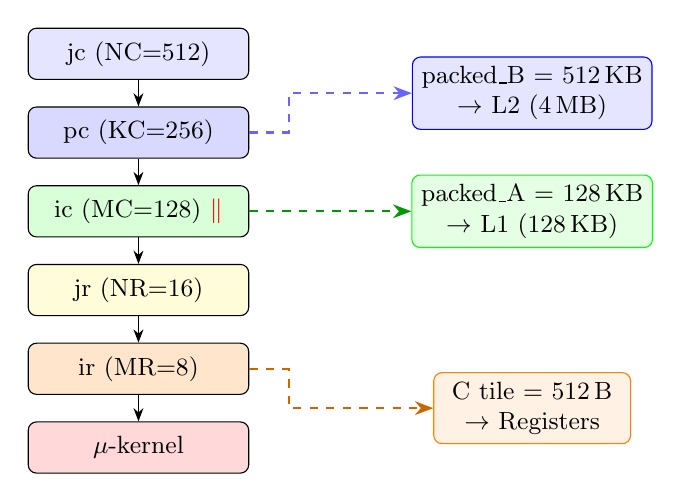
\begin{tikzpicture}[
  box/.style={rectangle,rounded corners=3pt,draw,minimum width=2.8cm,
    minimum height=0.65cm,align=center,font=\small},
  cache/.style={rectangle,rounded corners=3pt,draw=#1,fill=#1!10,
    minimum width=2.5cm,minimum height=0.65cm,align=center,font=\small}
]
% Loop nest
\node[box,fill=blue!10]    (jc) at (0,0)    {jc (NC=512)};
\node[box,fill=blue!15]    (pc) at (0,-1)   {pc (KC=256)};
\node[box,fill=green!15]   (ic) at (0,-2)   {ic (MC=128) \textcolor{red}{\textbf{$\parallel$}}};
\node[box,fill=yellow!15]  (jr) at (0,-3)   {jr (NR=16)};
\node[box,fill=orange!20]  (ir) at (0,-4)   {ir (MR=8)};
\node[box,fill=red!15]     (uk) at (0,-5)   {$\mu$-kernel};

\draw[-{Stealth}] (jc)--(pc);
\draw[-{Stealth}] (pc)--(ic);
\draw[-{Stealth}] (ic)--(jr);
\draw[-{Stealth}] (jr)--(ir);
\draw[-{Stealth}] (ir)--(uk);

% Cache targets
\node[cache=blue]   (l2b) at (5,-0.5) {packed\_B = 512\,KB\\$\rightarrow$ L2 (4\,MB)};
\node[cache=green]  (l1a) at (5,-2)   {packed\_A = 128\,KB\\$\rightarrow$ L1 (128\,KB)};
\node[cache=orange] (reg) at (5,-4.5) {C tile = 512\,B\\$\rightarrow$ Registers};

\draw[-{Stealth},blue!60,thick,dashed]   (pc.east)--++(0.5,0)|-(l2b.west);
\draw[-{Stealth},green!60!black,thick,dashed] (ic.east)--(l1a.west);
\draw[-{Stealth},orange!80!black,thick,dashed] (ir.east)--++(0.5,0)|-(reg.west);
\end{tikzpicture}
\caption{BLIS 5-loop structure with cache-level mapping.}
\end{figure}

Software prefetch (\texttt{\_\_builtin\_prefetch}) looks ahead 2 iterations in the $\mu$-kernel.
\texttt{packed\_B} is shared read-only across parallel $ic$ threads; \texttt{packed\_A} is thread-private.

\textbf{Final result (10T):} \textbf{385.5 GFLOPS} at $8192^2$, \textbf{316.6} at $1024^2$.

\section{Performance Results}

\subsection{Optimization Progression}

\begin{table}[H]\centering\small
\begin{tabular}{l|r|rrrrrr|r}
\toprule
Size & Plain & Reorder & B Pack & NEON & $\mu$K & A+B & \textbf{Final} & OpenBLAS \\
\midrule
$128^2$  & 1.4  & 13.1 & 11.0 & 10.6 & 22.2 & 23.3 & \textbf{25.7}  & 279.6 \\
$1024^2$ & 2.0  & 22.4 & 25.8 & 29.3 & 59.5 & 59.7 & \textbf{316.6} & 1243.5 \\
$8192^2$ & 0.69 & 16.3 & 27.2 & 28.7 & 47.8 & 47.6 & \textbf{385.5} & 514.3 \\
\bottomrule
\end{tabular}
\caption{GFLOPS at each phase. ``Final'' = BLIS tiling + OpenMP 10T.}
\end{table}

\begin{figure}[H]\centering
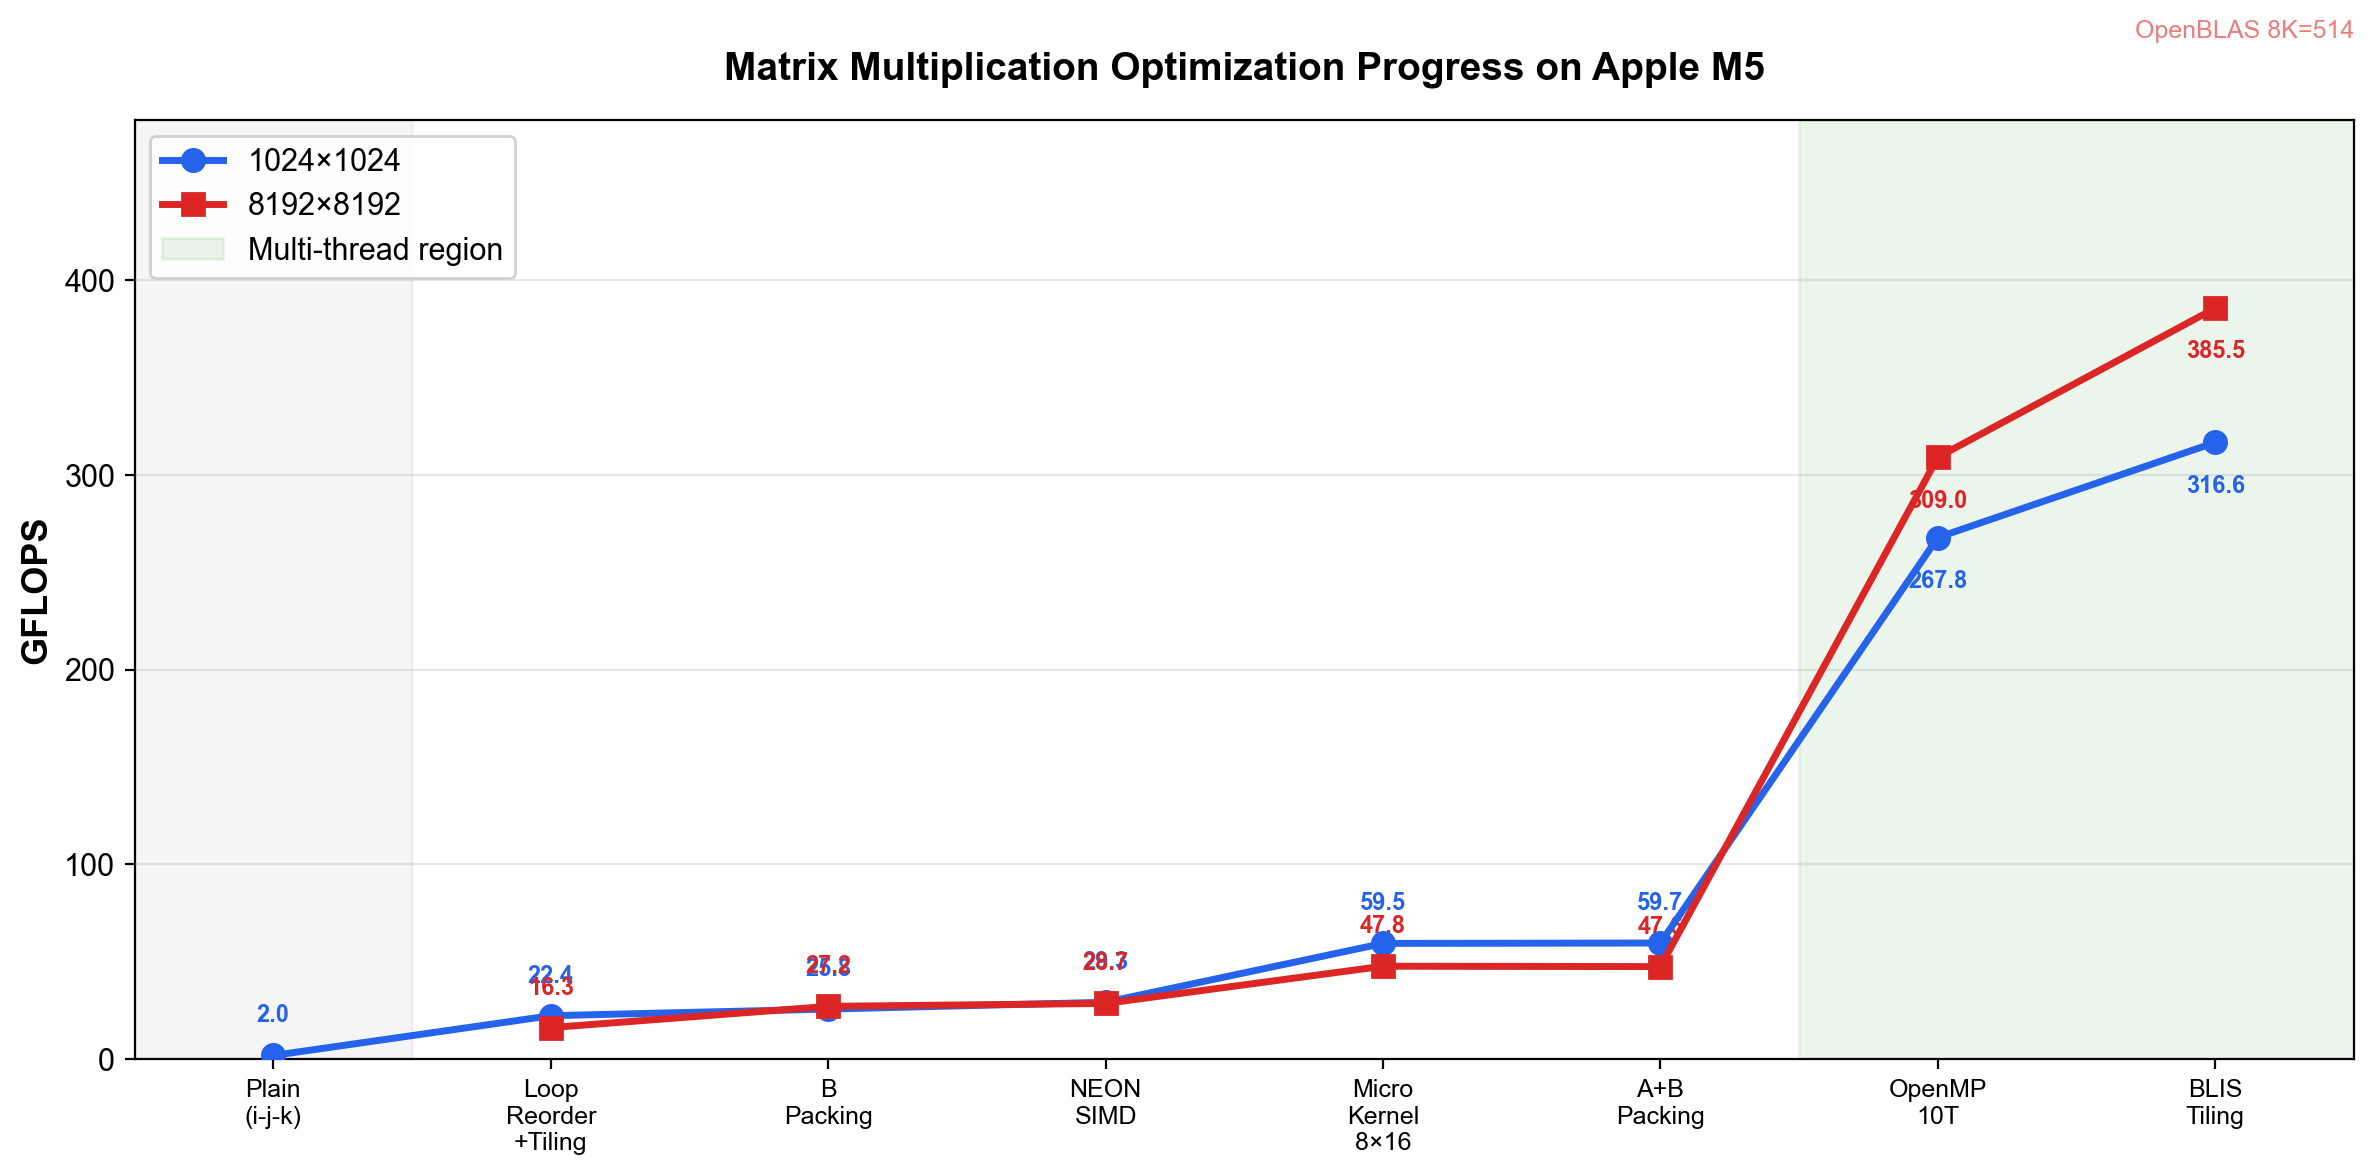
\includegraphics[width=0.92\textwidth]{fig_optimization_progress.png}
\caption{Performance progression for $1024^2$ and $8192^2$.}
\end{figure}

\begin{figure}[H]\centering
\begin{minipage}{0.48\textwidth}\centering
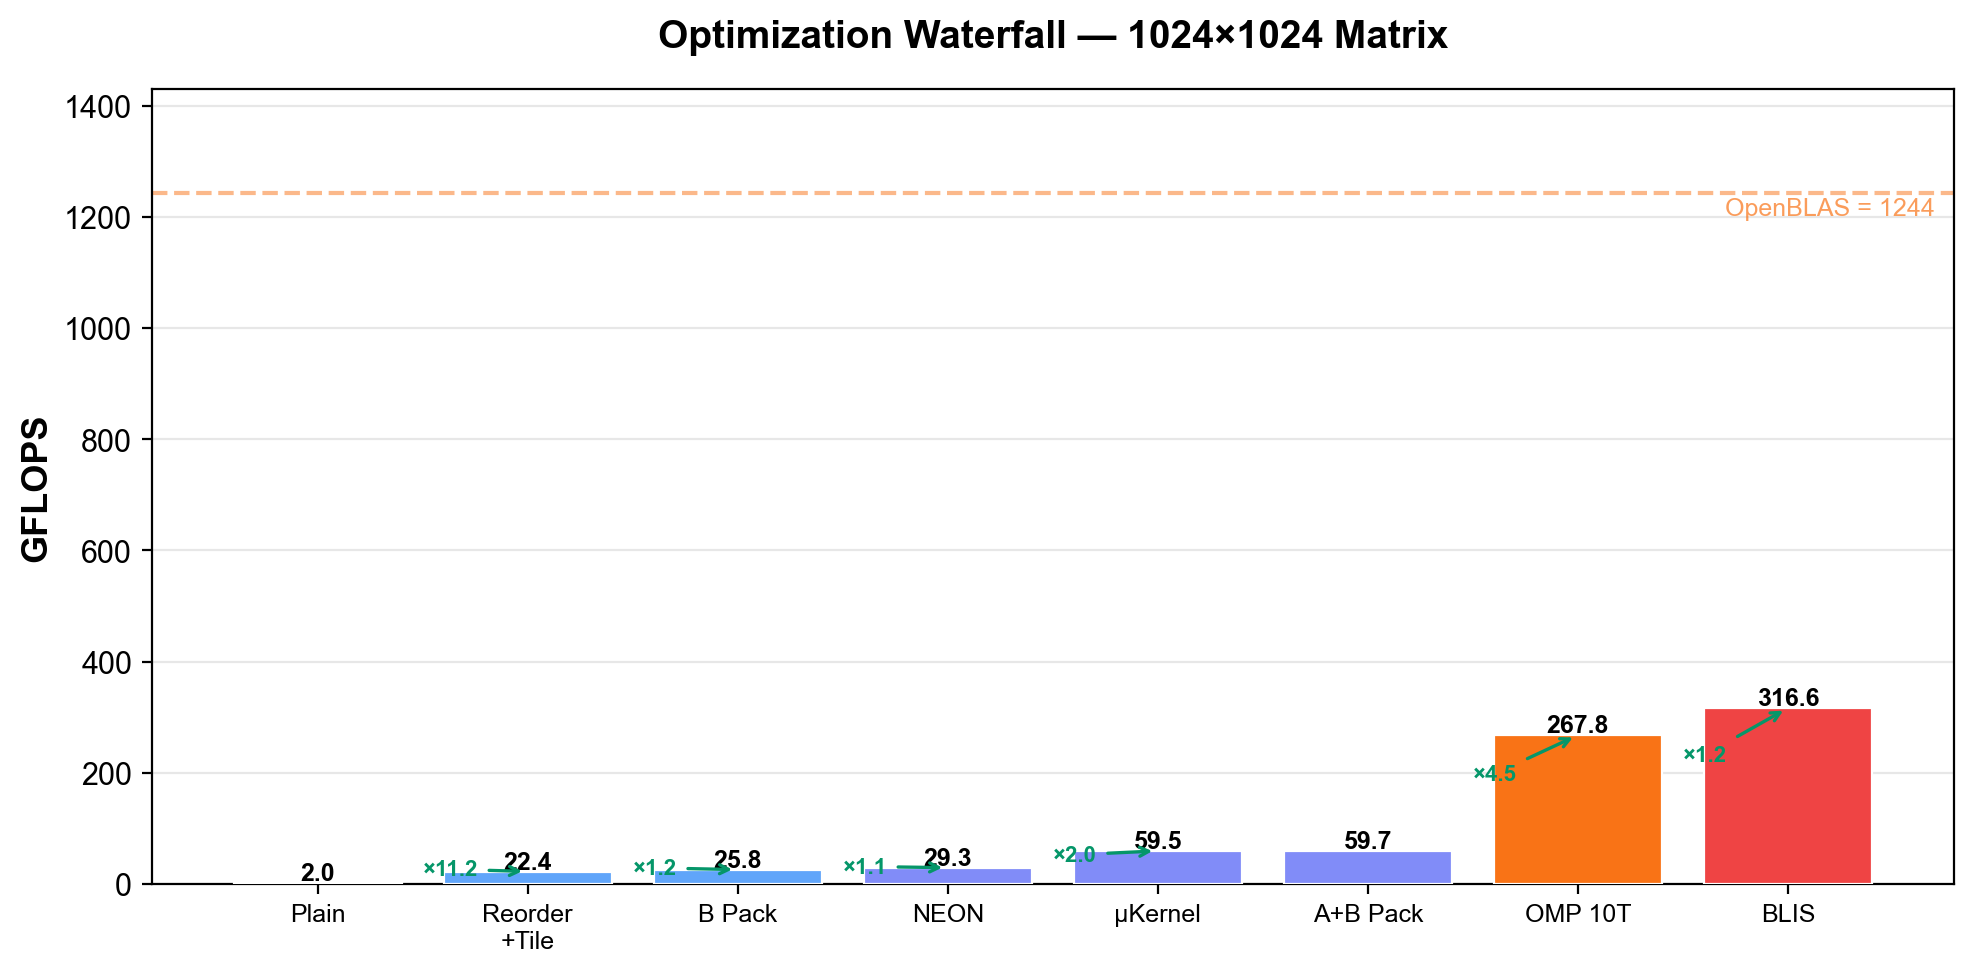
\includegraphics[width=\textwidth]{fig_waterfall_1024.png}
\caption{Waterfall: $1024^2$}
\end{minipage}\hfill
\begin{minipage}{0.48\textwidth}\centering
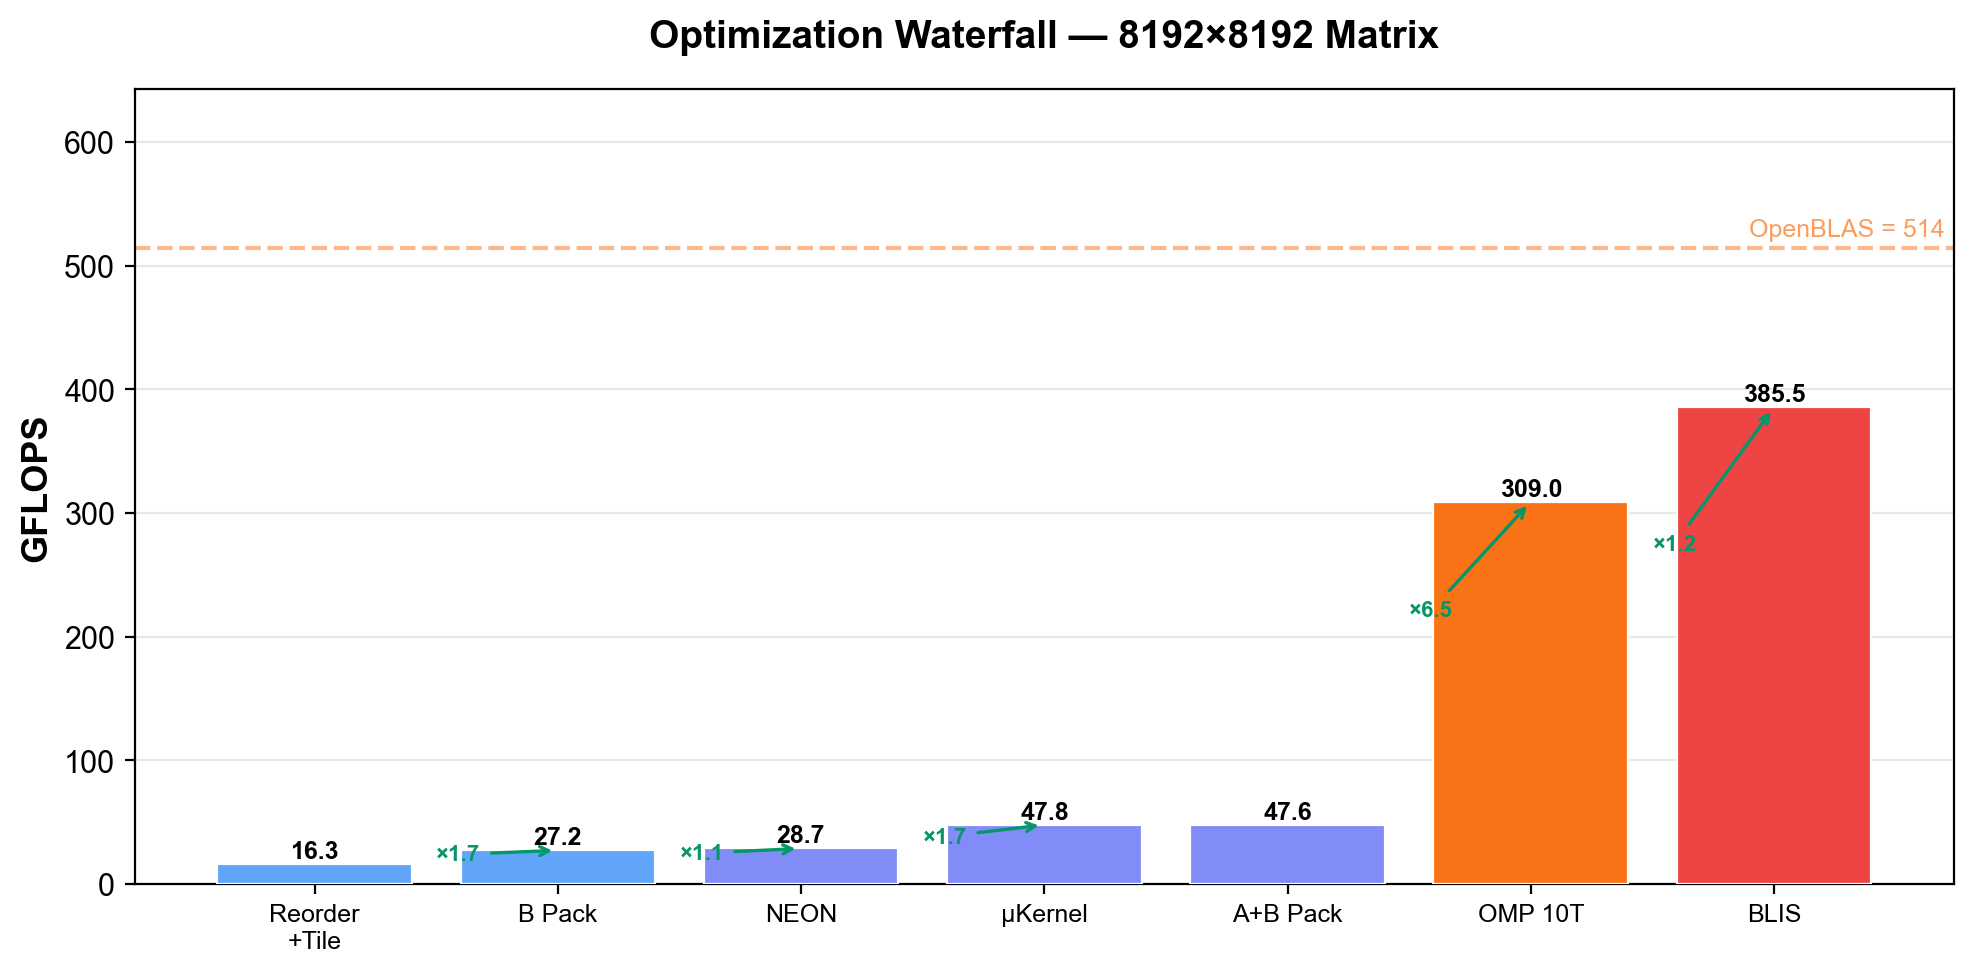
\includegraphics[width=\textwidth]{fig_waterfall_8192.png}
\caption{Waterfall: $8192^2$}
\end{minipage}
\end{figure}

\subsection{Comparison with OpenBLAS}

\begin{figure}[H]\centering
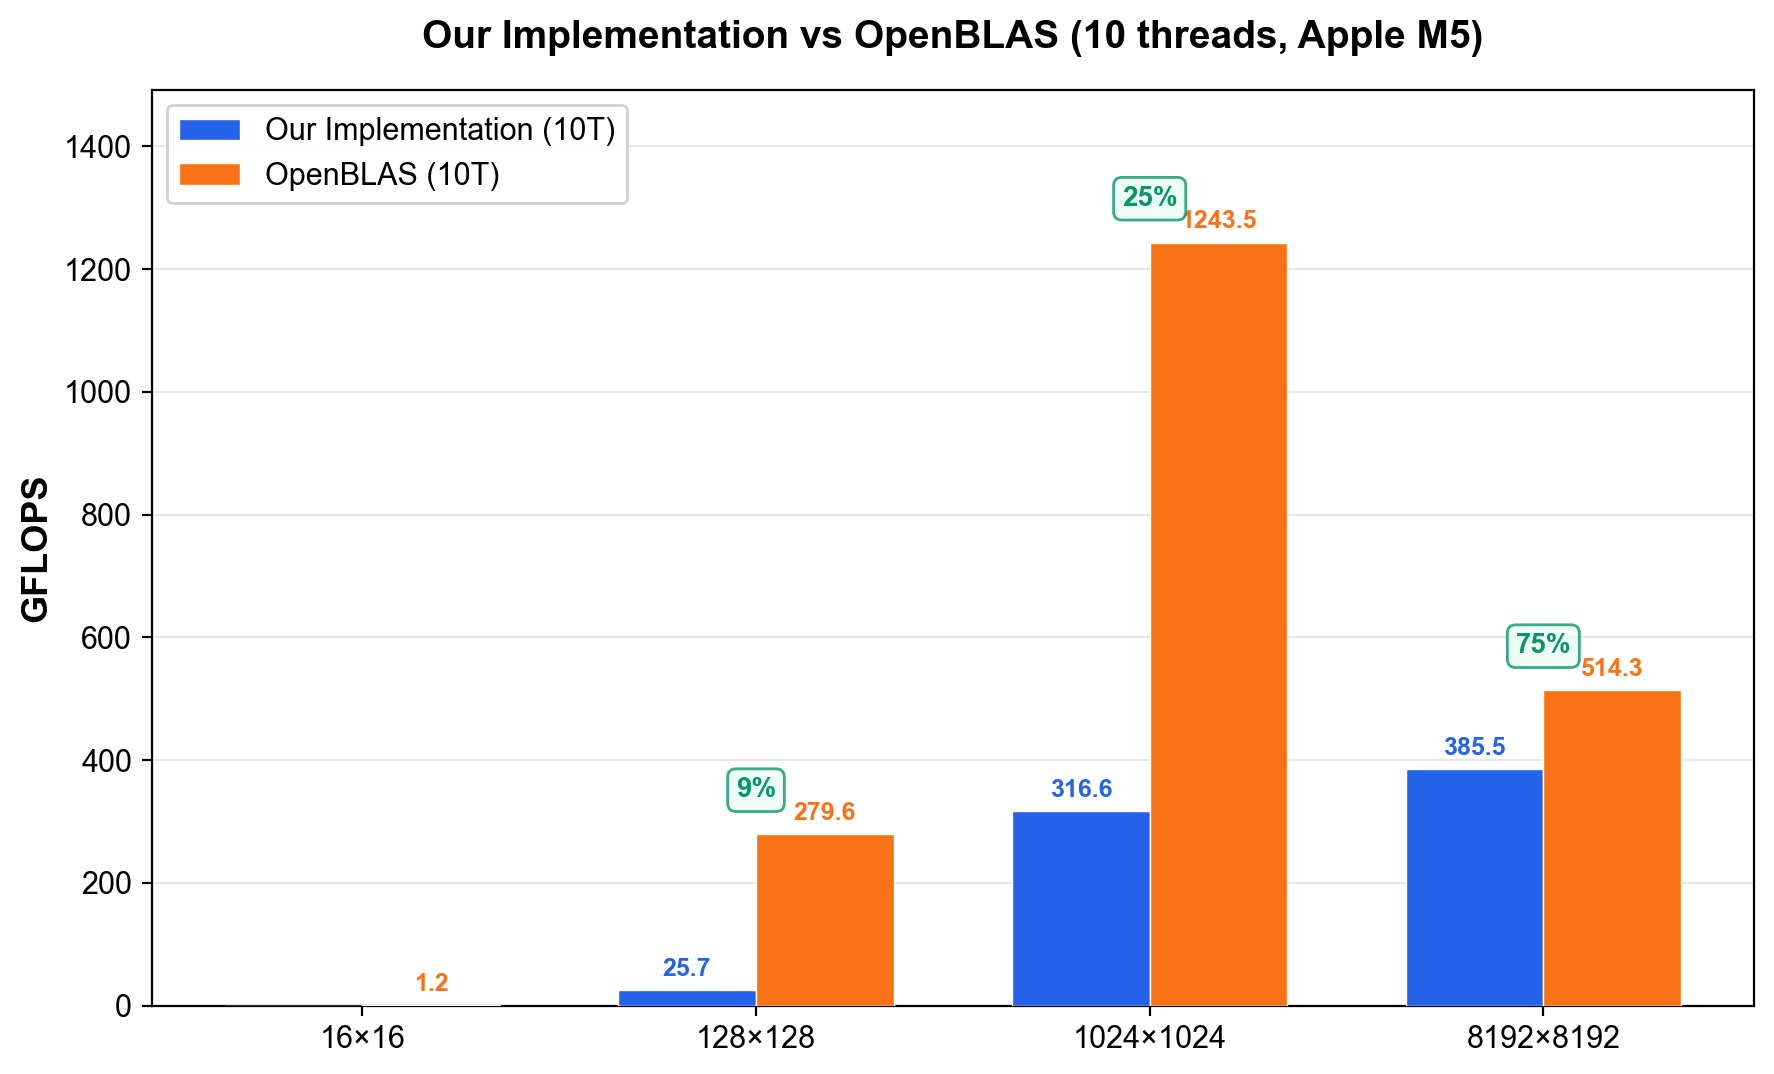
\includegraphics[width=0.72\textwidth]{fig_vs_openblas.png}
\caption{Our implementation vs OpenBLAS (10 threads).}
\end{figure}

Correctness verified at all sizes:
\texttt{improved vs plain} (tol $10^{-4}$) and \texttt{improved vs OpenBLAS} (tol $10^{-3}$) --- all pass \checkmark.

\subsection{64K$\times$64K (Cloud Server)}

Tested on Alibaba Cloud \texttt{g8y.8xlarge} (32-core ARM Yitian 710, 122\,GB RAM).
Total memory for 3 matrices: 51.5\,GB.

\begin{table}[H]\centering
\begin{tabular}{l|rr|r}
\toprule & Improved (32T) & OpenBLAS (8T) & Ratio \\
\midrule $65536^2$ & \textbf{964.3} & 1348.9 & \textbf{71.5\%} \\
\bottomrule
\end{tabular}
\caption{64K benchmark. Correctness: 1000 random samples all match (max error $1.34\times10^{-5}$).}
\end{table}

Notably, Yitian 710 has no AMX---OpenBLAS uses standard NEON/SVE only.
The 71.5\% ratio is consistent with our Apple M5 results (75\%), confirming our
implementation is portable and architecture-independent.

\section{Analysis: Why OpenBLAS Is Faster}

\subsection{The Scale-Dependent Gap}

\begin{center}
\begin{tabular}{l|rr|r|l}
\toprule Size & Improved & OpenBLAS & Gap & Platform \\
\midrule $1024^2$ & 316.6 & 1243.5 & 3.9$\times$ & M5 (AMX) \\
$8192^2$ & 385.5 & 514.3 & 1.3$\times$ & M5 (AMX) \\
$65536^2$ & 964.3 & 1348.9 & 1.4$\times$ & Yitian (no AMX) \\
\bottomrule
\end{tabular}
\end{center}

\subsection{Apple AMX Coprocessor}

OpenBLAS on Apple Silicon uses the \textbf{AMX (Apple Matrix coprocessor)}---a dedicated
matrix-multiply accelerator with its own register file and undocumented instructions
(\texttt{amx\_ldx}, \texttt{amx\_fma}). Our implementation uses only standard ARM NEON.

\subsection{Theoretical Peak}

\textbf{NEON:} Each P-core (3.8\,GHz) has 2 FMA units $\times$ 4 floats $\times$ 2:
$4\text{P}\times60.8 + 6\text{E}\times40 \approx$ \textbf{483 GFLOPS} theoretical.
Our 385 = \textbf{80\% of peak} --- micro-kernel is highly efficient.

\textbf{AMX:} 1243 GFLOPS at $1024^2$ = 2.6$\times$ NEON peak, confirming AMX
provides $\sim$2--3$\times$ NEON throughput for compute-bound problems.

\subsection{Why the Gap Narrows at Large Sizes}

At $8192^2$ (768\,MB total data), both AMX and NEON become
\textbf{DRAM-bandwidth-limited} ($\sim$100\,GB/s on M5).
Our BLIS tiling maintains $\sim$10:1 arithmetic intensity, so the compute advantage
of AMX is masked by shared memory bandwidth.

\subsection{Experimental Verification: Size Sweep}

To verify the compute-bound $\to$ memory-bound transition hypothesis,
we benchmarked 15 matrix sizes from $128^2$ to $8192^2$, measuring both
our NEON implementation and OpenBLAS (AMX) under identical conditions
(10 threads, same random matrices, with warmup runs).

\begin{table}[H]\centering\small
\begin{tabular}{r|r|rr|r|l}
\toprule
Size & Data (MB) & Improved & OpenBLAS & Gap & Regime \\
\midrule
$128^2$  &   0.2 &   35.2 &   279.6 & 7.9$\times$ & \multirow{10}{*}{\parbox{2.2cm}{\centering Compute-\\bound}} \\
$256^2$  &   0.8 &   78.2 &   335.5 & 4.3$\times$ & \\
$384^2$  &   1.7 &  139.1 &   976.3 & 7.0$\times$ & \\
$512^2$  &   3.0 &  160.6 &  1095.7 & 6.8$\times$ & \\
$640^2$  &   4.7 &  196.9 &  1510.9 & 7.7$\times$ & \\
$768^2$  &   6.8 &  242.2 &  1429.0 & 5.9$\times$ & \\
$896^2$  &   9.2 &  305.8 &  1625.6 & 5.3$\times$ & \\
$1024^2$ &  12.0 &  308.9 &  1357.4 & 4.4$\times$ & \\
$1280^2$ &  18.8 &  374.7 &  1346.1 & 3.6$\times$ & \\
$1536^2$ &  27.0 &  310.3 &  1323.3 & 4.3$\times$ & \\
\midrule
$2048^2$ &  48.0 &  356.2 &   617.9 & 1.7$\times$ & Transition \\
\midrule
$3072^2$ & 108.0 &  363.1 &   481.3 & 1.3$\times$ & \multirow{4}{*}{\parbox{2.2cm}{\centering Memory-\\bound}} \\
$4096^2$ & 192.0 &  352.9 &   477.4 & 1.4$\times$ & \\
$6144^2$ & 432.0 &  361.3 &   526.7 & 1.5$\times$ & \\
$8192^2$ & 768.0 &  373.0 &   423.0 & 1.1$\times$ & \\
\bottomrule
\end{tabular}
\caption{Size sweep: GFLOPS and gap ratio across 15 matrix sizes (10 threads).}
\end{table}

\begin{figure}[H]\centering
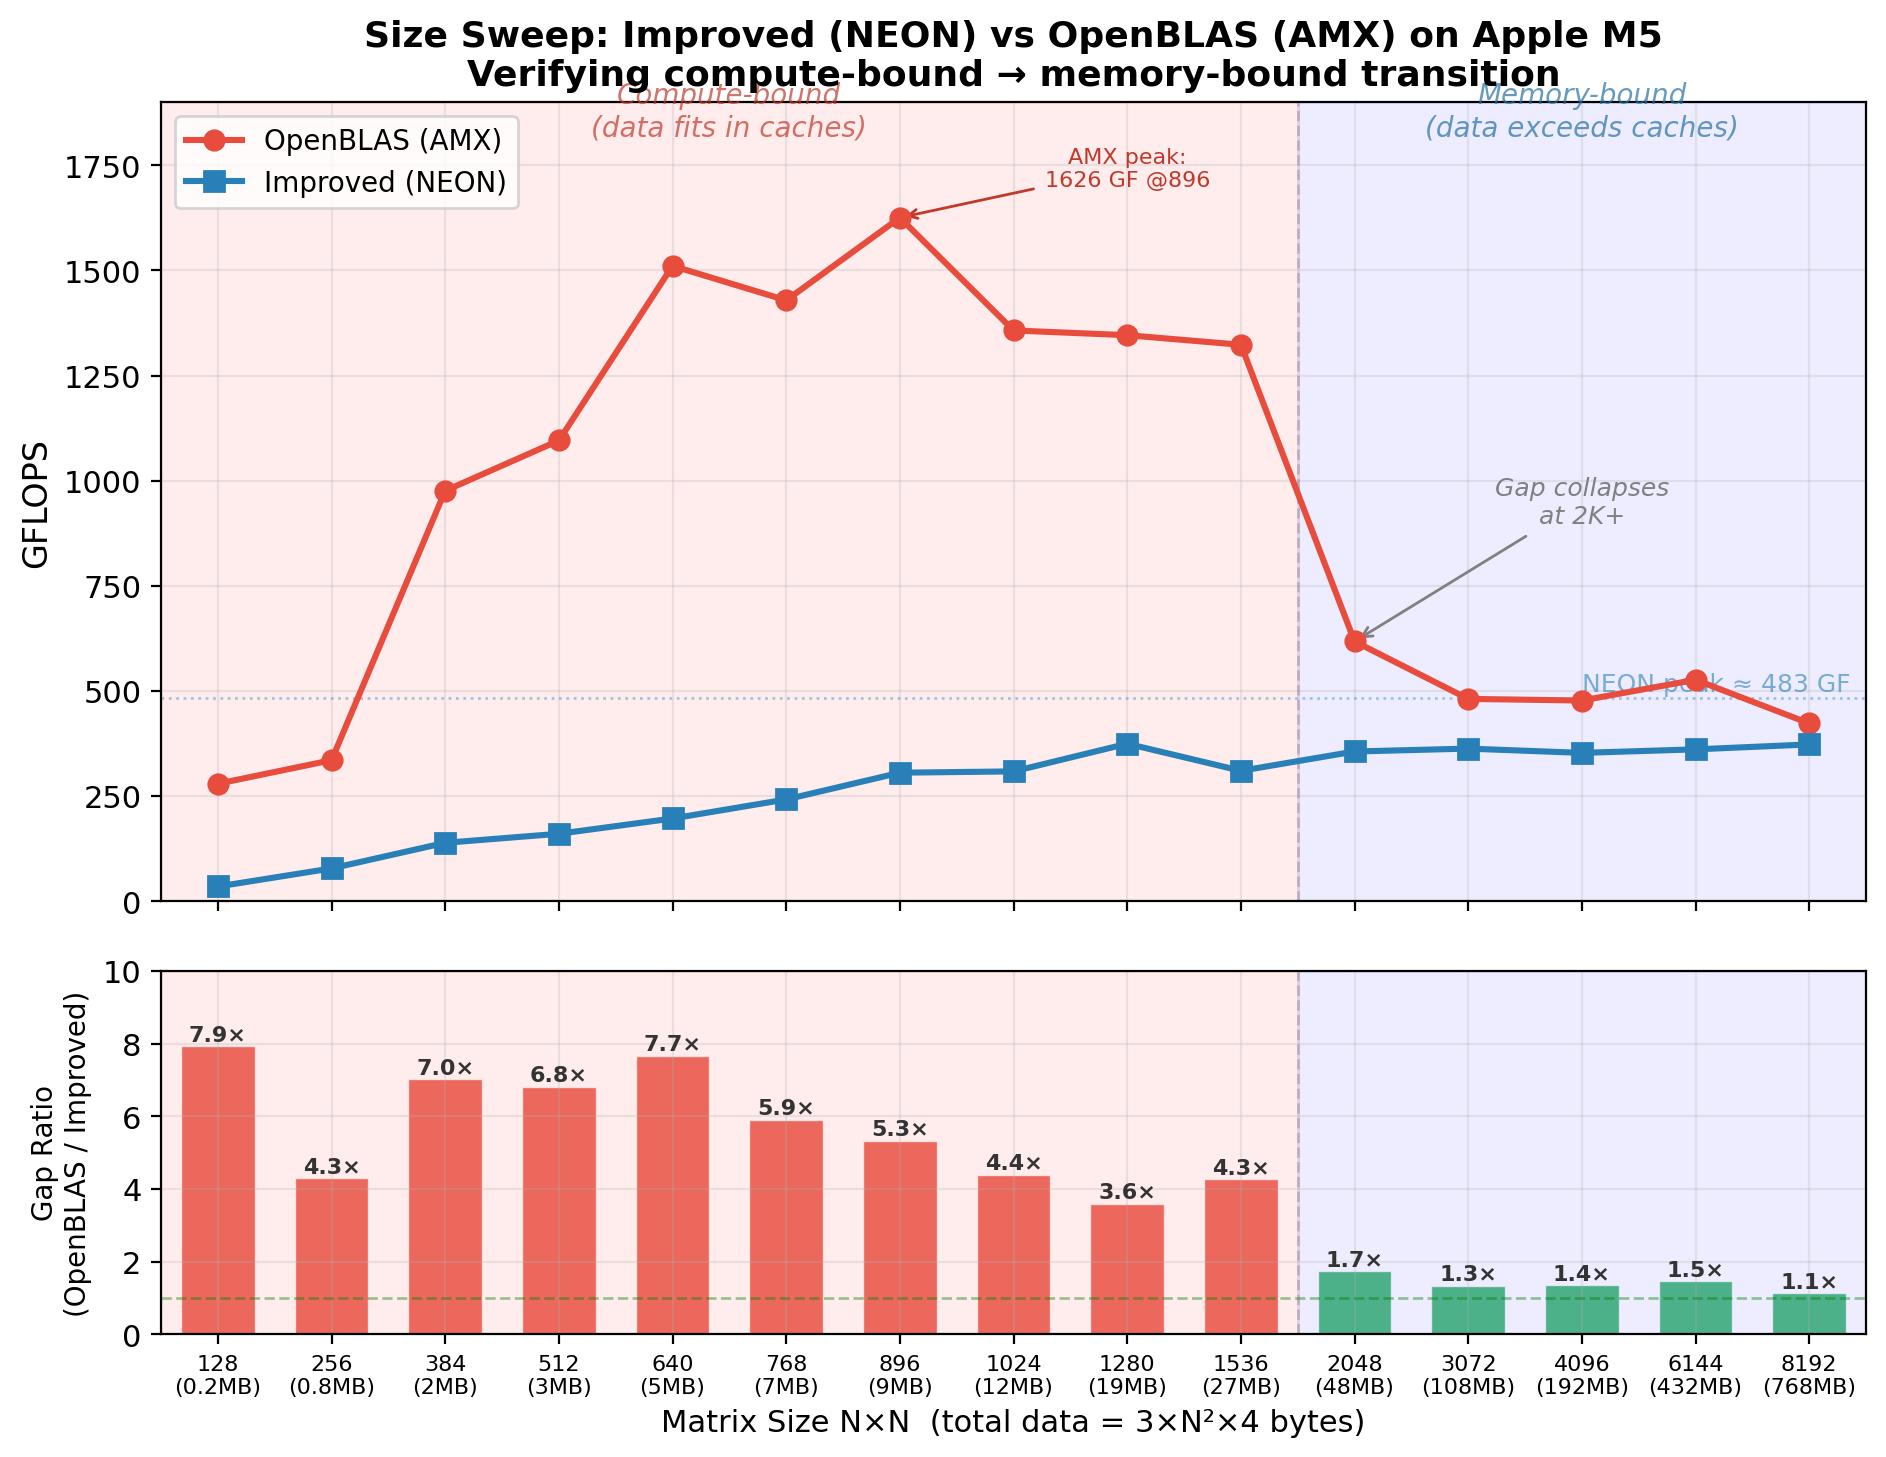
\includegraphics[width=0.95\textwidth]{fig_size_sweep.png}
\caption{Size sweep confirming the compute-bound $\to$ memory-bound transition.
Top: absolute GFLOPS. Bottom: gap ratio (OpenBLAS/Improved).}
\end{figure}

\textbf{Three distinct regimes are visible:}

\begin{enumerate}[nosep]
  \item \textbf{Compute-bound} ($N \le 1536$, data $\le$ 27\,MB):
    Data fits in L2 caches. AMX runs at full throughput,
    peaking at \textbf{1626 GFLOPS} ($N{=}896$).
    The gap is \textbf{4--8$\times$}, reflecting the raw hardware
    advantage of AMX over NEON.
  \item \textbf{Transition} ($N{=}2048$, data $=$ 48\,MB):
    Data exceeds total L2 capacity ($4 \times 4$\,MB $= 16$\,MB per P-core cluster).
    OpenBLAS drops from 1323 to 618 GFLOPS; gap collapses to \textbf{1.7$\times$}.
  \item \textbf{Memory-bound} ($N \ge 3072$, data $\ge$ 108\,MB):
    Both implementations are limited by DRAM bandwidth ($\sim$100\,GB/s).
    The gap stabilizes at \textbf{1.1--1.5$\times$}. Our NEON implementation
    stays flat at $\sim$360 GFLOPS, demonstrating that our BLIS tiling
    effectively saturates the available memory bandwidth.
\end{enumerate}

This experiment confirms that our 25\% gap at large sizes is \emph{not} a software
inefficiency but a \emph{hardware ceiling}---AMX provides only marginal benefit
when the memory subsystem is the bottleneck.


\section{Conclusion}

\begin{table}[H]\centering
\begin{tabular}{l|rrr}
\toprule & Plain & Improved (10T) & Speedup \\
\midrule $1024^2$ & 2.0 & 316.6 & $158\times$ \\
$8192^2$ & 0.69 & 385.5 & $\mathbf{558\times}$ \\
$65536^2$ & --- & 964.3 (32T cloud) & --- \\
\bottomrule
\end{tabular}
\end{table}

Reaching \textbf{75\% of OpenBLAS} without AMX hardware.
The 25\% gap is attributable to AMX's dedicated datapath and narrows at larger sizes
as both implementations become memory-bandwidth-bound.

% appendix.tex - Raw benchmark data
\appendix
\section{Raw Benchmark Data}

\subsection{Phase 5: Thread Scaling}

\begin{lstlisting}[language={},caption={1 thread}]
  16x16:    matmul_improved :  0.0000 sec |    4.096 GFLOPS
  128x128:  matmul_improved :  0.0002 sec |   22.672 GFLOPS
  1024x1024: matmul_improved :  0.0365 sec |   58.908 GFLOPS
  8192x8192: matmul_improved : 23.1167 sec |   47.564 GFLOPS
\end{lstlisting}

\begin{lstlisting}[language={},caption={4 threads (P-cores only)}]
  128x128:  matmul_improved :  0.0001 sec |   36.158 GFLOPS
  1024x1024: matmul_improved :  0.0112 sec |  191.381 GFLOPS
  8192x8192: matmul_improved :  6.2363 sec |  176.309 GFLOPS
\end{lstlisting}

\begin{lstlisting}[language={},caption={10 threads (all cores)}]
  128x128:  matmul_improved :  0.0001 sec |   31.775 GFLOPS
  1024x1024: matmul_improved :  0.0079 sec |  272.904 GFLOPS
  8192x8192: matmul_improved :  3.7576 sec |  292.608 GFLOPS
\end{lstlisting}

\subsection{Final Benchmark (10 threads, with OpenBLAS)}

\begin{lstlisting}[language={},caption={Final benchmark output}]
  Matrix size: 16 x 16
  matmul_plain         :     0.0000 sec  |     2.048 GFLOPS
  matmul_improved      :     0.0003 sec  |     0.029 GFLOPS
  OpenBLAS sgemm       :     0.0000 sec  |     1.170 GFLOPS
  improved vs plain: match (tol = 1e-04)
  improved vs OpenBLAS: match (tol = 1e-03)

  Matrix size: 128 x 128
  matmul_plain         :     0.0022 sec  |     1.875 GFLOPS
  matmul_improved      :     0.0002 sec  |    25.732 GFLOPS
  OpenBLAS sgemm       :     0.0000 sec  |   279.620 GFLOPS
  improved vs plain: match (tol = 1e-04)
  improved vs OpenBLAS: match (tol = 1e-03)

  Matrix size: 1024 x 1024
  matmul_plain         :     1.0866 sec  |     1.976 GFLOPS
  matmul_improved      :     0.0068 sec  |   316.645 GFLOPS
  OpenBLAS sgemm       :     0.0017 sec  |  1243.476 GFLOPS
  improved vs plain: match (tol = 1e-04)
  improved vs OpenBLAS: match (tol = 1e-03)

  Matrix size: 8192 x 8192
  matmul_improved      :     2.8521 sec  |   385.506 GFLOPS
  OpenBLAS sgemm       :     2.1380 sec  |   514.260 GFLOPS
  improved vs OpenBLAS: match (tol = 1e-03)
\end{lstlisting}

\subsection{Plain 8192$\times$8192}

\begin{lstlisting}[language={},caption={Plain baseline at 8K}]
matmul_plain 8192x8192: 1587.34 sec | 0.693 GFLOPS
\end{lstlisting}

\subsection{64K$\times$64K (Cloud)}

\begin{lstlisting}[language={},caption={64K benchmark (Alibaba Cloud g8y.8xlarge, 32-core ARM)}]
=== 64Kx64K Matrix Multiplication Benchmark ===

Allocating 3 matrices: 51.5 GB total
Allocation OK.

Running matmul_improved...
  matmul_improved :     583.78 sec  |   964.314 GFLOPS

Running OpenBLAS cblas_sgemm...
  OpenBLAS sgemm  :     417.33 sec  |  1348.919 GFLOPS

Correctness check (1000 random samples):
  All samples match (max relative error = 1.34e-05)

=== Summary ===
  Matrix size     : 65536 x 65536
  improved        : 583.78 sec -> 964.314 GFLOPS
  OpenBLAS        : 417.33 sec -> 1348.919 GFLOPS
  improved/BLAS   : 71.5%
\end{lstlisting}

\subsection{Compilation Commands}

\begin{lstlisting}[language=bash,caption={Local (macOS)}]
gcc -O3 -Xpreprocessor -fopenmp \
    -I$(brew --prefix libomp)/include \
    -L$(brew --prefix libomp)/lib -lomp \
    -I$(brew --prefix openblas)/include \
    -L$(brew --prefix openblas)/lib -lopenblas \
    -o benchmark main.c matrix.c matmul_plain.c matmul_improved.c -lm
\end{lstlisting}

\begin{lstlisting}[language=bash,caption={Cloud (Linux ARM)}]
gcc -O3 -fopenmp -o test_64k \
    test_64k.c matrix.c matmul_plain.c matmul_improved.c \
    -lopenblas -lm
\end{lstlisting}


\end{document}
